% -------------------------------------------------------------------------
% ------ nuweb macros (redefine as desired, or omit with "nuweb -p") ------
% -------------------------------------------------------------------------
\providecommand{\NWtxtMacroDefBy}{Macro defined by}
\providecommand{\NWtxtMacroRefIn}{Macro referenced in}
\providecommand{\NWtxtMacroNoRef}{Macro never referenced}
\providecommand{\NWtxtDefBy}{Defined by}
\providecommand{\NWtxtRefIn}{Referenced in}
\providecommand{\NWtxtNoRef}{Not referenced}
\providecommand{\NWtxtFileDefBy}{File defined by}
\providecommand{\NWsep}{${\diamond}$}
\providecommand{\NWlink}[2]{\hyperlink{#1}{#2}}
\providecommand{\NWtarget}[2]{% move baseline up by \baselineskip 
  \raisebox{\baselineskip}[1.5ex][0ex]{%
    \mbox{%
      \hypertarget{#1}{%
        \raisebox{-1\baselineskip}[0ex][0ex]{%
          \mbox{#2}%
}}}}}
% -------------------------------------------------------------------------

\documentclass[11pt,oneside]{article}	%use"amsart"insteadof"article"forAMSLaTeXformat
\usepackage{geometry}		%Seegeometry.pdftolearnthelayoutoptions.Therearelots.
\geometry{letterpaper}		%...ora4paperora5paperor...
%\geometry{landscape}		%Activateforforrotatedpagegeometry
%\usepackage[parfill]{parskip}		%Activatetobeginparagraphswithanemptylineratherthananindent
\usepackage{graphicx}				%Usepdf,png,jpg,orepsßwithpdflatex;useepsinDVImode
								%TeXwillautomaticallyconverteps-->pdfinpdflatex		
\usepackage{amssymb}
\usepackage[colorlinks]{hyperref}

\usepackage{framed}
\usepackage{amsthm}
\newtheorem{remark}{Remark}
\newtheorem{definition}{Definition}

%----macros begin---------------------------------------------------------------
\usepackage{color}
\usepackage{amsthm}

\def\conv{\mbox{\textrm{conv}\,}}
\def\aff{\mbox{\textrm{aff}\,}}
\def\E{\mathbb{E}}
\def\R{\mathbb{R}}
\def\Z{\mathbb{Z}}
\def\tex{\TeX}
\def\latex{\LaTeX}
\def\v#1{{\bf #1}}
\def\p#1{{\bf #1}}
\def\T#1{{\bf #1}}

\def\vet#1{{\left(\begin{array}{cccccccccccccccccccc}#1\end{array}\right)}}
\def\mat#1{{\left(\begin{array}{cccccccccccccccccccc}#1\end{array}\right)}}

\def\lin{\mbox{\rm lin}\,}
\def\aff{\mbox{\rm aff}\,}
\def\pos{\mbox{\rm pos}\,}
\def\cone{\mbox{\rm cone}\,}
\def\conv{\mbox{\rm conv}\,}
\newcommand{\homog}[0]{\mbox{\rm homog}\,}
\newcommand{\relint}[0]{\mbox{\rm relint}\,}

%----macros end-----------------------------------------------------------------

\title{Imaging Morphology with LAR
\footnote{This document is part of the \emph{Linear Algebraic Representation with CoChains} (LAR-CC) framework~\cite{cclar-proj:2013:00}. \today}
}
\author{Alberto Paoluzzi}
%\date{}							%Activatetodisplayagivendateornodate

\begin{document}
\maketitle
\nonstopmode

\begin{abstract}
In this module we aim to implement the four operators of mathematical morphology, i.e.~the \emph{dilation}, \emph{erosion}, \emph{opening} and \emph{closing} operators, by the way of matrix operations representing the linear operators---\emph{boundary} and \emph{coboundary}---over LAR. 
According to the multidimensional character of LAR, our implementation is dimension-independent.
In few words, it works as follows: (a)  the input is (the coordinate representation of) a $d$-chain $\gamma$; (b) compute its boundary $\partial_d(\gamma)$; (c) extract the maximal $(d-2)$-chain $\epsilon \subset \partial_d(\gamma)$; (d) consider the $(d-1)$-chain returned from its coboundary $\delta_{d-2}(\epsilon)$; (e) compute the $d$-chain $\eta := \delta_{d-1}(\delta_{d-2}(\epsilon)) \subset C_d$ \emph{without} performing the  $\mbox{mod\ 2}$ final transformation on the resulting coordinate vector, that would provide a zero result, according to the standard algebraic constraint $\delta\circ\delta=0$. It is easy to show that $\eta \equiv (\oplus \gamma) - (\ominus \gamma)$ provides the \emph{morphological gradient} operator. The four standard morphological operators are therefore  consequently computable.
\end{abstract}

\tableofcontents

\section{Test image generation}

Various methods for the input or the generation of a test image  are developed in the subsections of this section. The aim is to prepare a set of controlled test beds, used to check both the implementation and the working properties of our topological implementation of morphological operators. 


\subsection{Random binary multidimensional image}

A multidimensional binary image is generated here by using a random approach, both for the bulk structure and the small artefacts of the image.  


%-------------------------------------------------------------------------------
\begin{flushleft} \small
\begin{minipage}{\linewidth} \label{scrap1}
\protect\makebox[0ex][r]{\NWtarget{nuweb2a}{\rule{0ex}{0ex}}\hspace{1em}}$\langle\,$Generation of random image\nobreak\ {\footnotesize 2a}$\,\rangle\equiv$
\vspace{-1ex}
\begin{list}{}{} \item
\mbox{}\verb@@\\
\mbox{}\verb@def randomImage(shape, structure, noiseFraction=0.0):@\\
\mbox{}\verb@   """ Generation of random image of given shape and structure. @\\
\mbox{}\verb@      Return scipy.ndarray(shape)@\\
\mbox{}\verb@   """@\\
\mbox{}\verb@   print "noiseFraction =",noiseFraction@\\
\mbox{}\verb@   @\hbox{$\langle\,$Generation of bulk array structure\nobreak\ {\footnotesize \NWlink{nuweb2b}{2b}}$\,\rangle$}\verb@@\\
\mbox{}\verb@   @\hbox{$\langle\,$Generation of random artifacts\nobreak\ {\footnotesize \NWlink{nuweb3a}{3a}}$\,\rangle$}\verb@@\\
\mbox{}\verb@   return image_array@\\
\mbox{}\verb@@{\NWsep}
\end{list}
\vspace{-1ex}
\footnotesize\addtolength{\baselineskip}{-1ex}
\begin{list}{}{\setlength{\itemsep}{-\parsep}\setlength{\itemindent}{-\leftmargin}}
\item \NWtxtMacroRefIn\ \NWlink{nuweb14e}{14e}.
\end{list}
\end{minipage}\\[4ex]
\end{flushleft}
%-------------------------------------------------------------------------------


\paragraph{Generation of the gross image}
First we generate a 2D grid of squares by Cartesian product, and produce the bulk of the random image then used to test our approach to morphological operators via topological ones.


%import scipy
%scipy.misc.imsave('outfile.jpg', image_array)
%
%scipy.ndimage.imread(fname, flatten=False, mode=None)[source]
%
%rand(10, 10)
%
	
%-------------------------------------------------------------------------------
\begin{flushleft} \small
\begin{minipage}{\linewidth} \label{scrap2}
\protect\makebox[0ex][r]{\NWtarget{nuweb2b}{\rule{0ex}{0ex}}\hspace{1em}}$\langle\,$Generation of bulk array structure\nobreak\ {\footnotesize 2b}$\,\rangle\equiv$
\vspace{-1ex}
\begin{list}{}{} \item
\mbox{}\verb@ranges = [shape[k]/structure[k] for k in range(len(shape))]@\\
\mbox{}\verb@random_array = randint(0, 255, size=structure)@\\
\mbox{}\verb@image_array = numpy.zeros(shape)@\\
\mbox{}\verb@for index in scipy.array(CART(AA(range)(shape))):@\\
\mbox{}\verb@   block = index/ranges@\\
\mbox{}\verb@   if random_array[tuple(block)] < 127:@\\
\mbox{}\verb@      image_array[tuple(index)] = 0 @\\
\mbox{}\verb@   else: @\\
\mbox{}\verb@      image_array[tuple(index)] = 255@\\
\mbox{}\verb@@{\NWsep}
\end{list}
\vspace{-1ex}
\footnotesize\addtolength{\baselineskip}{-1ex}
\begin{list}{}{\setlength{\itemsep}{-\parsep}\setlength{\itemindent}{-\leftmargin}}
\item \NWtxtMacroRefIn\ \NWlink{nuweb2a}{2a}.
\end{list}
\end{minipage}\\[4ex]
\end{flushleft}
%-------------------------------------------------------------------------------



\paragraph{Generation of random artefacts upon the image}

Then random noise is added to the previously generated image, in order to produce artifacts at the pixel scale. 

%-------------------------------------------------------------------------------
\begin{flushleft} \small
\begin{minipage}{\linewidth} \label{scrap3}
\protect\makebox[0ex][r]{\NWtarget{nuweb3a}{\rule{0ex}{0ex}}\hspace{1em}}$\langle\,$Generation of random artifacts\nobreak\ {\footnotesize 3a}$\,\rangle\equiv$
\vspace{-1ex}
\begin{list}{}{} \item
\mbox{}\verb@noiseQuantity = PROD(list(shape))*noiseFraction@\\
\mbox{}\verb@k = 0@\\
\mbox{}\verb@while k < noiseQuantity:@\\
\mbox{}\verb@   index = tuple(AA(randint)(list(shape)))@\\
\mbox{}\verb@   if image_array[index] == 0: image_array[index] = 255@\\
\mbox{}\verb@   else: image_array[index] = 0@\\
\mbox{}\verb@   k += 1@\\
\mbox{}\verb@if len(shape)==3:@\\
\mbox{}\verb@   for k in range(shape[0]):@\\
\mbox{}\verb@      scipy.misc.imsave('tmp/outfile'+str(k).zfill(3)+'.png', image_array[k])@\\
\mbox{}\verb@else:@\\
\mbox{}\verb@   scipy.misc.imsave('tmp/outfile'+str(k).zfill(3)+'.png', image_array)@\\
\mbox{}\verb@@{\NWsep}
\end{list}
\vspace{-1ex}
\footnotesize\addtolength{\baselineskip}{-1ex}
\begin{list}{}{\setlength{\itemsep}{-\parsep}\setlength{\itemindent}{-\leftmargin}}
\item \NWtxtMacroRefIn\ \NWlink{nuweb2a}{2a}.
\end{list}
\end{minipage}\\[4ex]
\end{flushleft}
%-------------------------------------------------------------------------------


\section{Selection of an image segment}

In this section we implement several methods for image segmentation and segment selection. 

\subsection{Selection of a test chain}

The first and simplest method is the selection of the portion of a binary image contained within a masking window.
Here we select the (white) sub-image contained in a given window, and compute the coordinate representation of the (chain) sub-image.

\paragraph{Mask definition}

A \emph{window} within a $d$-image is defined by $2\times d$ integer numbers (2 multi-indices), corresponding to the window  \texttt{minPoint} (minimum indices) and to the window \texttt{maxPoint} (maximum indices). A list of multi-index tuples, contained in the \texttt{window} variable, is generated by the function \texttt{setMaskWindow} below.

%-------------------------------------------------------------------------------
\begin{flushleft} \small
\begin{minipage}{\linewidth} \label{scrap4}
\protect\makebox[0ex][r]{\NWtarget{nuweb3b}{\rule{0ex}{0ex}}\hspace{1em}}$\langle\,$Generation of a masking window\nobreak\ {\footnotesize 3b}$\,\rangle\equiv$
\vspace{-1ex}
\begin{list}{}{} \item
\mbox{}\verb@def setMaskWindow(window,image_array):@\\
\mbox{}\verb@   minPoint, maxPoint = window@\\
\mbox{}\verb@   imageShape = list(image_array.shape)@\\
\mbox{}\verb@   @\hbox{$\langle\,$Generation of multi-index window\nobreak\ {\footnotesize \NWlink{nuweb4}{4}}$\,\rangle$}\verb@@\\
\mbox{}\verb@   @\hbox{$\langle\,$Window-to-chain mapping\nobreak\ {\footnotesize \NWlink{nuweb5b}{5b}}$\,\rangle$}\verb@@\\
\mbox{}\verb@   @\hbox{$\langle\,$Change chain color to grey\nobreak\ {\footnotesize \NWlink{nuweb5c}{5c}}$\,\rangle$}\verb@@\\
\mbox{}\verb@   return segmentChain@\\
\mbox{}\verb@@{\NWsep}
\end{list}
\vspace{-1ex}
\footnotesize\addtolength{\baselineskip}{-1ex}
\begin{list}{}{\setlength{\itemsep}{-\parsep}\setlength{\itemindent}{-\leftmargin}}
\item \NWtxtMacroRefIn\ \NWlink{nuweb14e}{14e}.
\end{list}
\end{minipage}\\[4ex]
\end{flushleft}
%-------------------------------------------------------------------------------

The set of tuples of indices contained in a (multidimensional) window is given below.
 
%-------------------------------------------------------------------------------
\begin{flushleft} \small
\begin{minipage}{\linewidth} \label{scrap5}
\protect\makebox[0ex][r]{\NWtarget{nuweb4}{\rule{0ex}{0ex}}\hspace{1em}}$\langle\,$Generation of multi-index window\nobreak\ {\footnotesize 4}$\,\rangle\equiv$
\vspace{-1ex}
\begin{list}{}{} \item
\mbox{}\verb@indexRanges = zip(minPoint,maxPoint)@\\
\mbox{}\verb@tuples = CART([range(min,max) for min,max in indexRanges])@\\
\mbox{}\verb@@{\NWsep}
\end{list}
\vspace{-1ex}
\footnotesize\addtolength{\baselineskip}{-1ex}
\begin{list}{}{\setlength{\itemsep}{-\parsep}\setlength{\itemindent}{-\leftmargin}}
\item \NWtxtMacroRefIn\ \NWlink{nuweb3b}{3b}.
\end{list}
\end{minipage}\\[4ex]
\end{flushleft}
%-------------------------------------------------------------------------------



\subsection{Mapping of integer tuples to integers}

In order to produce the coordinate representation of a chain in a multidimensional image (or $d$-image) we need: (a) to choose a basis of image elements, i.e.~of $d$-cells, and in particular to fix an ordering of them; (b) to map the multidimensional index, selecting a single $d$-cell of the image, to a single integer mapping the cell to its linear position within the chosen basis ordering. 


\paragraph{Grid of hyper-cubes of unit size}
Let $S_i=(0,1,...,n_i-1)$ be ordered integer sets with $n_i$ elements, and 
\[
S= S_0 \times S_1 \times \cdots \times S_{d-1}
\] 
the set of indices of elements of a $d$-image.

\begin{definition}[$d$-image shape]
The \emph{shape} of a $d$-image with $n_0\times n_1 \times\cdots\times n_{d-1}$ elements (here called \emph{voxels}) is the ordered set $(n_0, n_1, \ldots, n_{d-1})$.
\end{definition}


\paragraph{$d$-dimensional row-major order}

Given a $d$-image with shape $S=(n_0,n_1,...,n_{d-1})$ and number of elements $n=\prod n_i$, 
the mapping  
\[
S_0 \times S_1 \times \cdots \times S_{d-1} \to \{ 0, 1, \ldots, n-1\}
\]
 is a {linear combination} with integer {weights}  $(w_0,w_1,...,w_{d-2},1)$, such that:
\[
(i_0,i_1,...,i_{d-1}) \mapsto i_0 w_0 +i_1 w_1 +\cdots +i_{d-1} w_{d-1},
\]
where 
\[
w_k = n_{k+1}  n_{k+2} \cdots  n_{d-1}, \qquad 0\leq k\leq d-2.
\]

\paragraph{Implementation}
A functional implementation of the \emph{Tuples to integers mapping} is given by the second-order  \texttt{mapTupleToInt} function, that  accepts in a first application the \texttt{shape} of the image (to compute the tuple space of indices of $d$-cells), and then takes a single tuple in the second application. Of course, the function  returns the cell address in the linear address space associated to the given \texttt{shape}.

%-------------------------------------------------------------------------------
\begin{flushleft} \small
\begin{minipage}{\linewidth} \label{scrap6}
\protect\makebox[0ex][r]{\NWtarget{nuweb5a}{\rule{0ex}{0ex}}\hspace{1em}}$\langle\,$Tuples to integers mapping\nobreak\ {\footnotesize 5a}$\,\rangle\equiv$
\vspace{-1ex}
\begin{list}{}{} \item
\mbox{}\verb@def mapTupleToInt(shape):@\\
\mbox{}\verb@   d = len(shape)@\\
\mbox{}\verb@   weights = [PROD(shape[(k+1):]) for k in range(d-1)]+[1]@\\
\mbox{}\verb@   @\\
\mbox{}\verb@   def mapTupleToInt0(tuple):@\\
\mbox{}\verb@      return INNERPROD([tuple,weights])@\\
\mbox{}\verb@   return mapTupleToInt0@\\
\mbox{}\verb@@{\NWsep}
\end{list}
\vspace{-1ex}
\footnotesize\addtolength{\baselineskip}{-1ex}
\begin{list}{}{\setlength{\itemsep}{-\parsep}\setlength{\itemindent}{-\leftmargin}}
\item \NWtxtMacroRefIn\ \NWlink{nuweb14e}{14e}.
\end{list}
\end{minipage}\\[4ex]
\end{flushleft}
%-------------------------------------------------------------------------------


\paragraph{From tuples multi-indices to chain coordinates}

The set of address \texttt{tuples} of $d-cells$ ($d$-dimensional image elements) within the \emph{mask} is here mapped to the corresponding set of (single) integers associated to the low-level image elements (pixels or voxels, depending on the image dimension and shape), denoted \texttt{windowChain}. Such total chain of the mask \texttt{window} is then filtered to contain the only coordinates of \emph{white} image elements within the window, and returned as the set of integer cell indices \texttt{segmentChain}.


%-------------------------------------------------------------------------------
\begin{flushleft} \small
\begin{minipage}{\linewidth} \label{scrap7}
\protect\makebox[0ex][r]{\NWtarget{nuweb5b}{\rule{0ex}{0ex}}\hspace{1em}}$\langle\,$Window-to-chain mapping\nobreak\ {\footnotesize 5b}$\,\rangle\equiv$
\vspace{-1ex}
\begin{list}{}{} \item
\mbox{}\verb@imageCochain = image_array.reshape(PROD(imageShape))@\\
\mbox{}\verb@mapping = mapTupleToInt(imageShape)@\\
\mbox{}\verb@windowChain = [mapping(tuple) for tuple in tuples]@\\
\mbox{}\verb@segmentChain = [cell for cell in windowChain if imageCochain[cell]==255]@\\
\mbox{}\verb@@{\NWsep}
\end{list}
\vspace{-1ex}
\footnotesize\addtolength{\baselineskip}{-1ex}
\begin{list}{}{\setlength{\itemsep}{-\parsep}\setlength{\itemindent}{-\leftmargin}}
\item \NWtxtMacroRefIn\ \NWlink{nuweb3b}{3b}.
\end{list}
\end{minipage}\\[4ex]
\end{flushleft}
%-------------------------------------------------------------------------------

\subsection{Show segment chain on binary image}

Now we need to show visually the selected \texttt{segmentChain}, by change the color of its cells from white (255) to middle grey (127). Just remember that \texttt{imageCochain} is the linear representation of the image, with number of cells equal to \texttt{PROD(imageShape)}. Then the modified image is restored within \texttt{image\_array}, and is finally exported to a \texttt{.png} image file.

%-------------------------------------------------------------------------------
\begin{flushleft} \small
\begin{minipage}{\linewidth} \label{scrap8}
\protect\makebox[0ex][r]{\NWtarget{nuweb5c}{\rule{0ex}{0ex}}\hspace{1em}}$\langle\,$Change chain color to grey\nobreak\ {\footnotesize 5c}$\,\rangle\equiv$
\vspace{-1ex}
\begin{list}{}{} \item
\mbox{}\verb@for cell in segmentChain: imageCochain[cell] = 127@\\
\mbox{}\verb@image_array = imageCochain.reshape(imageShape)@\\
\mbox{}\verb@#for k in range(shape[0]):@\\
\mbox{}\verb@#  scipy.misc.imsave('tmp/outfile'+str(k).zfill(3)+'.png', image_array[k])@\\
\mbox{}\verb@@{\NWsep}
\end{list}
\vspace{-1ex}
\footnotesize\addtolength{\baselineskip}{-1ex}
\begin{list}{}{\setlength{\itemsep}{-\parsep}\setlength{\itemindent}{-\leftmargin}}
\item \NWtxtMacroRefIn\ \NWlink{nuweb3b}{3b}.
\end{list}
\end{minipage}\\[4ex]
\end{flushleft}
%-------------------------------------------------------------------------------


\section{Construction of (co)boundary operators}

A $d$-image is a \emph{cellular $d$-complex} where cells are $k$-cuboids ($0\leq k\leq d$), i.e.~Cartesian products of a number $k$ of 1D intervals, embedded in $d$-dimensional Euclidean space. 


\subsection{Reading and writing LAR of image from disk}
Since the construction of the \emph{chain complex} supported by a cellular complex with $O(n^d)$ $d$-cells---and $n=O(10^3)$---may be really time-consuming, it is unquestionably useful to store on disk, once and for all, the topological model of a multidimensional image, i.e.~the LAR of its chain complex,  and just restore it (or the needed part of it --- TODO) when necessary, since \emph{it only depends on the \texttt{shape} of a $d$-image}, i.e.~from the array arrangement of its $d$-cells (``hypervoxels'').

%-------------------------------------------------------------------------------
\begin{flushleft} \small
\begin{minipage}{\linewidth} \label{scrap9}
\protect\makebox[0ex][r]{\NWtarget{nuweb6}{\rule{0ex}{0ex}}\hspace{1em}}$\langle\,$Save and restore data object from file\nobreak\ {\footnotesize 6}$\,\rangle\equiv$
\vspace{-1ex}
\begin{list}{}{} \item
\mbox{}\verb@def dump(object,filename):@\\
\mbox{}\verb@   with open(filename, 'wb') as f:@\\
\mbox{}\verb@       pickle.dump(object, f)@\\
\mbox{}\verb@       @\\
\mbox{}\verb@def load(filename):@\\
\mbox{}\verb@   with open(filename, 'rb') as f:@\\
\mbox{}\verb@       object = pickle.load(f)@\\
\mbox{}\verb@   return object@\\
\mbox{}\verb@@{\NWsep}
\end{list}
\vspace{-1ex}
\footnotesize\addtolength{\baselineskip}{-1ex}
\begin{list}{}{\setlength{\itemsep}{-\parsep}\setlength{\itemindent}{-\leftmargin}}
\item \NWtxtMacroRefIn\ \NWlink{nuweb14e}{14e}.
\end{list}
\end{minipage}\\[4ex]
\end{flushleft}
%-------------------------------------------------------------------------------


%-------------------------------------------------------------------------------
\begin{flushleft} \small
\begin{minipage}{\linewidth} \label{scrap10}
\protect\makebox[0ex][r]{\NWtarget{nuweb7a}{\rule{0ex}{0ex}}\hspace{1em}}$\langle\,$Save or restore the chain complex of multidimensional image\nobreak\ {\footnotesize 7a}$\,\rangle\equiv$
\vspace{-1ex}
\begin{list}{}{} \item
\mbox{}\verb@def imageChainComplex (shape):@\\
\mbox{}\verb@   tokens = str(shape)[1:-1].split(',')@\\
\mbox{}\verb@   tokens = [token.strip() for token in tokens]@\\
\mbox{}\verb@   filename = "tmp/larimage-" + "-".join(tokens) + ".pickle"@\\
\mbox{}\verb@   @\\
\mbox{}\verb@   if os.path.isfile(filename):@\\
\mbox{}\verb@      shape, skeletons, operators = loadImageLAR(filename)@\\
\mbox{}\verb@   else:@\\
\mbox{}\verb@      skeletons = gridSkeletons(list(shape))@\\
\mbox{}\verb@      operators = boundaryOps(skeletons)@\\
\mbox{}\verb@      imageLAR = (shape, skeletons, operators)@\\
\mbox{}\verb@      dump(imageLAR,filename)@\\
\mbox{}\verb@      print "filename =",filename@\\
\mbox{}\verb@   return shape, skeletons, operators@\\
\mbox{}\verb@   @\\
\mbox{}\verb@def loadImageLAR(filename):@\\
\mbox{}\verb@   object = load(filename)@\\
\mbox{}\verb@   shape, skeletons, operators = object@\\
\mbox{}\verb@   return shape, skeletons, operators@\\
\mbox{}\verb@@{\NWsep}
\end{list}
\vspace{-1ex}
\footnotesize\addtolength{\baselineskip}{-1ex}
\begin{list}{}{\setlength{\itemsep}{-\parsep}\setlength{\itemindent}{-\leftmargin}}
\item \NWtxtMacroRefIn\ \NWlink{nuweb14e}{14e}.
\end{list}
\end{minipage}\\[4ex]
\end{flushleft}
%-------------------------------------------------------------------------------
	



\subsection{LAR chain complex construction}

In our first multidimensional implementation of morphological operators through algebraic topology of the image seen as a cellular complex, we compute the whole sequence of characteristic matrices $M_k$ ($0\leq k \leq d$) in \texttt{BRC} form, and the whole sequence of matrices $[\partial_k]$ ($0\leq k \leq d$) in \texttt{CSR} form.

\begin{figure}[htbp] %  figure placement: here, top, bottom, or page
   \centering
   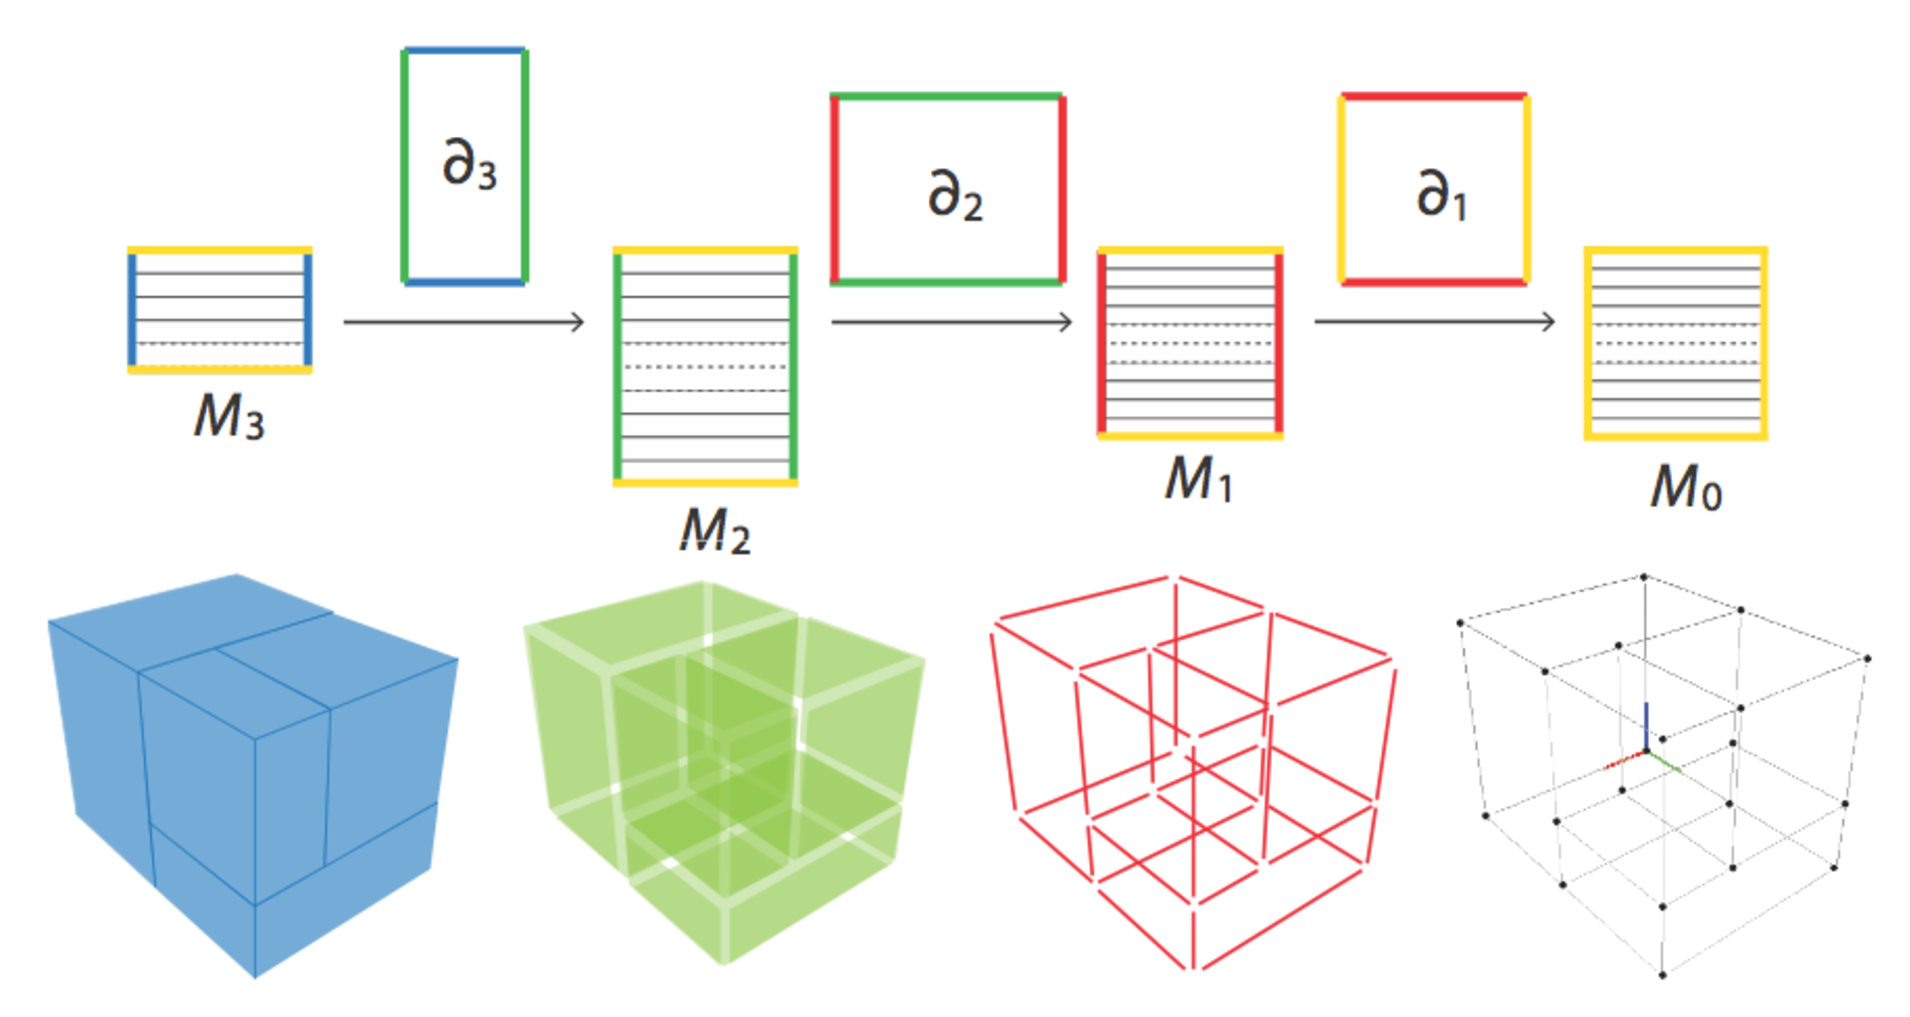
\includegraphics[width=0.7\linewidth]{images/larcomplex} 
   \caption{The LAR definition of  a chain complex: a sequence of characteristic matrices \emph{and} a sequence of boundary operators.}
   \label{fig:example}
\end{figure}

\paragraph{Array of characteristic matrices}

A direct construction of cuboidal complexes is offered, within the \texttt{larcc} package, by the \texttt{largrid.larCuboids} function. 

%-------------------------------------------------------------------------------
\begin{flushleft} \small
\begin{minipage}{\linewidth} \label{scrap11}
\protect\makebox[0ex][r]{\NWtarget{nuweb7b}{\rule{0ex}{0ex}}\hspace{1em}}$\langle\,$Characteristic matrices of multidimensional image\nobreak\ {\footnotesize 7b}$\,\rangle\equiv$
\vspace{-1ex}
\begin{list}{}{} \item
\mbox{}\verb@def larImage(shape):@\\
\mbox{}\verb@   """ Compute vertices and skeletons of an image of given shape """@\\
\mbox{}\verb@   imageVerts = larImageVerts(shape)@\\
\mbox{}\verb@   skeletons = gridSkeletons(list(shape))@\\
\mbox{}\verb@   return imageVerts, skeletons@\\
\mbox{}\verb@@{\NWsep}
\end{list}
\vspace{-1ex}
\footnotesize\addtolength{\baselineskip}{-1ex}
\begin{list}{}{\setlength{\itemsep}{-\parsep}\setlength{\itemindent}{-\leftmargin}}
\item \NWtxtMacroRefIn\ \NWlink{nuweb14e}{14e}.
\end{list}
\end{minipage}\\[4ex]
\end{flushleft}
%-------------------------------------------------------------------------------

\paragraph{Example}
Consider a (very!) small 3D image of \texttt{shape=(2,2,2)}. The data structures returned by the \texttt{larImage} function are shown below, where \texttt{imageVerts} gives the integer coordinates of vertices of the 3D (image) complex, and \texttt{skeletons} is the list of characteristic matrices $M_k$ ($0\leq k\leq d$) in \texttt{BRC} form.

%-------------------------------------------------------------------------------
\begin{flushleft} \small \label{scrap12}
\protect\makebox[0ex][r]{\NWtarget{nuweb8}{\rule{0ex}{0ex}}\hspace{1em}}$\langle\,$Example of characteristic matrices (and vertices) of multidimensional image\nobreak\ {\footnotesize 8}$\,\rangle\equiv$
\vspace{-1ex}
\begin{list}{}{} \item
\mbox{}\verb@imageVerts, skeletons = larImage((2,2,2))@\\
\mbox{}\verb@@\\
\mbox{}\verb@print imageVerts,@\\
\mbox{}\verb@>>> [[0,0,0],[0,0,1],[0,0,2],[0,1,0],[0,1,1],[0,1,2],[0,2,0],[0,2,1],[0,2,2],@\\
\mbox{}\verb@[1,0,0],[1,0,1],[1,0,2],[1,1,0],[1,1,1],[1,1,2],[1,2,0],[1,2,1],[1,2,2],[2,0,@\\
\mbox{}\verb@0],[2,0,1],[2,0,2],[2,1,0],[2,1,1],[2,1,2],[2,2,0],[2,2,1],[2,2,2]]@\\
\mbox{}\verb@@\\
\mbox{}\verb@print skeletons[1:],@\\
\mbox{}\verb@>>> [@\\
\mbox{}\verb@[[0,1],[1,2],[3,4],[4,5],[6,7],[7,8],[9,10],[10,11],[12,13],[13,14],[15,@\\
\mbox{}\verb@16],[16,17],[18,19],[19,20],[21,22],[22,23],[24,25],[25,26],[0,3],[1,4],[2,@\\
\mbox{}\verb@5],[3,6],[4,7],[5,8],[9,12],[10,13],[11,14],[12,15],[13,16],[14,17],[18,21],@\\
\mbox{}\verb@[19,22],[20,23],[21,24],[22,25],[23,26],[0,9],[1,10],[2,11],[3,12],[4,13],[5,@\\
\mbox{}\verb@14],[6,15],[7,16],[8,17],[9,18],[10,19],[11,20],[12,21],[13,22],[14,23],[15,@\\
\mbox{}\verb@24],[16,25],[17,26]],@\\
\mbox{}\verb@[[0,1,3,4],[1,2,4,5],[3,4,6,7],[4,5,7,8],[9,10,12,13],[10,11,13,14],[12,13,15,@\\
\mbox{}\verb@16],[13,14,16,17],[18,19,21,22],[19,20,22,23],[21,22,24,25],[22,23,25,26],[0,@\\
\mbox{}\verb@1,9,10],[1,2,10,11],[3,4,12,13],[4,5,13,14],[6,7,15,16],[7,8,16,17],[9,10,18,@\\
\mbox{}\verb@19],[10,11,19,20],[12,13,21,22],[13,14,22,23],[15,16,24,25],[16,17,25,26],[0,@\\
\mbox{}\verb@3,9,12],[1,4,10,13],[2,5,11,14],[3,6,12,15],[4,7,13,16],[5,8,14,17],[9,12,18,@\\
\mbox{}\verb@21],[10,13,19,22],[11,14,20,23],[12,15,21,24],[13,16,22,25],[14,17,23,26]],@\\
\mbox{}\verb@[[0,1,3,4,9,10,12,13],[1,2,4,5,10,11,13,14],[3,4,6,7,12,13,15,16],[4,5,7,8,13,@\\
\mbox{}\verb@14,16,17],[9,10,12,13,18,19,21,22],[10,11,13,14,19,20,22,23],[12,13,15,16,21,@\\
\mbox{}\verb@22,24,25],[13,14,16,17,22,23,25,26]]@\\
\mbox{}\verb@]@\\
\mbox{}\verb@@{\NWsep}
\end{list}
\vspace{-1ex}
\footnotesize\addtolength{\baselineskip}{-1ex}
\begin{list}{}{\setlength{\itemsep}{-\parsep}\setlength{\itemindent}{-\leftmargin}}
\item {\NWtxtMacroNoRef}.
\end{list}
\end{flushleft}
%-------------------------------------------------------------------------------


\paragraph{Array of matrices of boundary operators}

The function \texttt{boundaryOps} takes the array of \texttt{BRC} reprs of characteristic matrices, and returns the array of \texttt{CSR} matrix reprs of boundary operators $\partial_k$ ($1\leq k\leq d$).

%-------------------------------------------------------------------------------
\begin{flushleft} \small
\begin{minipage}{\linewidth} \label{scrap13}
\protect\makebox[0ex][r]{\NWtarget{nuweb9a}{\rule{0ex}{0ex}}\hspace{1em}}$\langle\,$CSR matrices of boundary operators\nobreak\ {\footnotesize 9a}$\,\rangle\equiv$
\vspace{-1ex}
\begin{list}{}{} \item
\mbox{}\verb@def boundaryOps(skeletons):@\\
\mbox{}\verb@   """ CSR matrices of boundary operators from list of skeletons """@\\
\mbox{}\verb@   return [boundary(skeletons[k+1],faces) @\\
\mbox{}\verb@      for k,faces in enumerate(skeletons[:-1])]@\\
\mbox{}\verb@@{\NWsep}
\end{list}
\vspace{-1ex}
\footnotesize\addtolength{\baselineskip}{-1ex}
\begin{list}{}{\setlength{\itemsep}{-\parsep}\setlength{\itemindent}{-\leftmargin}}
\item \NWtxtMacroRefIn\ \NWlink{nuweb14e}{14e}.
\end{list}
\end{minipage}\\[4ex]
\end{flushleft}
%-------------------------------------------------------------------------------


\paragraph{Boundary chain of a $k$-chain of a $d$-image}

%-------------------------------------------------------------------------------
\begin{flushleft} \small
\begin{minipage}{\linewidth} \label{scrap14}
\protect\makebox[0ex][r]{\NWtarget{nuweb9b}{\rule{0ex}{0ex}}\hspace{1em}}$\langle\,$Boundary of image chain computation\nobreak\ {\footnotesize 9b}$\,\rangle\equiv$
\vspace{-1ex}
\begin{list}{}{} \item
\mbox{}\verb@def imageChainBoundary(shape, operators):@\\
\mbox{}\verb@   imageVerts, skeletons = larImage(shape)@\\
\mbox{}\verb@   # operators = boundaryOps(skeletons)@\\
\mbox{}\verb@   cellNumber = PROD(list(shape))@\\
\mbox{}\verb@   @\\
\mbox{}\verb@   def imageChainBoundary0(k):@\\
\mbox{}\verb@      csrBoundaryMat = operators[-1]@\\
\mbox{}\verb@      facets = skeletons[k-1]@\\
\mbox{}\verb@      @\\
\mbox{}\verb@      def imageChainBoundary1(chain):@\\
\mbox{}\verb@         @\hbox{$\langle\,$Boundary*chain product and interpretation\nobreak\ {\footnotesize \NWlink{nuweb10a}{10a}}$\,\rangle$}\verb@@\\
\mbox{}\verb@         boundaryChainModel = imageVerts, [facets[h] for h in boundaryChain]     @\\
\mbox{}\verb@         return boundaryChainModel,boundaryChain@\\
\mbox{}\verb@      @\\
\mbox{}\verb@      return imageChainBoundary1@\\
\mbox{}\verb@   return imageChainBoundary0@\\
\mbox{}\verb@@{\NWsep}
\end{list}
\vspace{-1ex}
\footnotesize\addtolength{\baselineskip}{-1ex}
\begin{list}{}{\setlength{\itemsep}{-\parsep}\setlength{\itemindent}{-\leftmargin}}
\item \NWtxtMacroRefIn\ \NWlink{nuweb14e}{14e}.
\end{list}
\end{minipage}\\[4ex]
\end{flushleft}
%-------------------------------------------------------------------------------

\paragraph{Low-level SpMSpV matrix-chain product}

A low-level implementation of the product of boundary matrix times the coordinate representation of the image chain under consideration is given below. It was enveloped and protected in this macro because it is strongly dependent on the CSR structures and tools provided by the sparse matrix module of the \texttt{scipy} library.	

%-------------------------------------------------------------------------------
\begin{flushleft} \small
\begin{minipage}{\linewidth} \label{scrap15}
\protect\makebox[0ex][r]{\NWtarget{nuweb10a}{\rule{0ex}{0ex}}\hspace{1em}}$\langle\,$Boundary*chain product and interpretation\nobreak\ {\footnotesize 10a}$\,\rangle\equiv$
\vspace{-1ex}
\begin{list}{}{} \item
\mbox{}\verb@csrChain = scipy.sparse.csr_matrix((cellNumber,1))@\\
\mbox{}\verb@for h in chain: csrChain[h,0] = 1@\\
\mbox{}\verb@csrBoundaryChain = matrixProduct(csrBoundaryMat, csrChain)@\\
\mbox{}\verb@for h,value in enumerate(csrBoundaryChain.data):@\\
\mbox{}\verb@   if MOD([value,2]) == 0: csrBoundaryChain.data[h] = 0@\\
\mbox{}\verb@cooBoundaryChain = csrBoundaryChain.tocoo()@\\
\mbox{}\verb@boundaryChain = [cooBoundaryChain.row[h] @\\
\mbox{}\verb@   for h,val in enumerate(cooBoundaryChain.data) if val == 1]@\\
\mbox{}\verb@@{\NWsep}
\end{list}
\vspace{-1ex}
\footnotesize\addtolength{\baselineskip}{-1ex}
\begin{list}{}{\setlength{\itemsep}{-\parsep}\setlength{\itemindent}{-\leftmargin}}
\item \NWtxtMacroRefIn\ \NWlink{nuweb9b}{9b}.
\end{list}
\end{minipage}\\[4ex]
\end{flushleft}
%-------------------------------------------------------------------------------


\subsection{Visualisation of an image chain and its boundary}


\paragraph{$d$-Chain visualisation}

The \texttt{visImageChain} function given by the macro \emph{Visualisation of an image chain} below. 

%-------------------------------------------------------------------------------
\begin{flushleft} \small
\begin{minipage}{\linewidth} \label{scrap16}
\protect\makebox[0ex][r]{\NWtarget{nuweb10b}{\rule{0ex}{0ex}}\hspace{1em}}$\langle\,$Pyplasm visualisation of an image chain\nobreak\ {\footnotesize 10b}$\,\rangle\equiv$
\vspace{-1ex}
\begin{list}{}{} \item
\mbox{}\verb@def visImageChain (shape,chain, imageVerts, skeletons):@\\
\mbox{}\verb@   # imageVerts, skeletons = larImage(shape)@\\
\mbox{}\verb@   chainLAR = [cell for k,cell in enumerate(skeletons[-1]) if k in chain]@\\
\mbox{}\verb@   return imageVerts,chainLAR@\\
\mbox{}\verb@@{\NWsep}
\end{list}
\vspace{-1ex}
\footnotesize\addtolength{\baselineskip}{-1ex}
\begin{list}{}{\setlength{\itemsep}{-\parsep}\setlength{\itemindent}{-\leftmargin}}
\item \NWtxtMacroRefIn\ \NWlink{nuweb14e}{14e}.
\end{list}
\end{minipage}\\[4ex]
\end{flushleft}
%-------------------------------------------------------------------------------


\begin{figure}[htbp] %  figure placement: here, top, bottom, or page
   \centering
   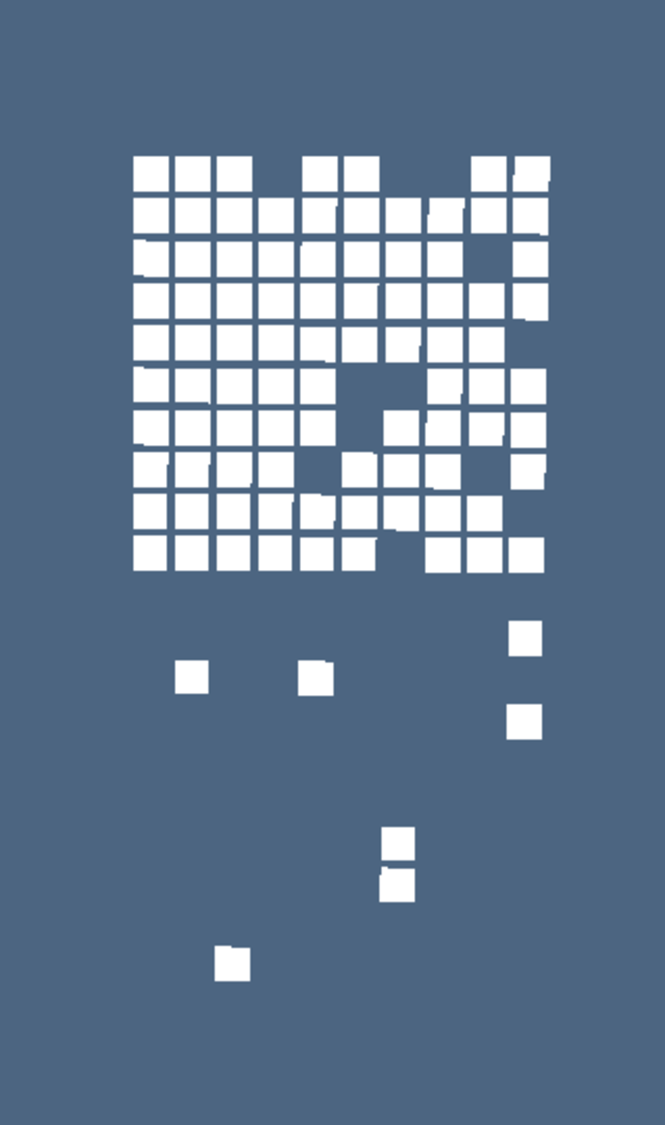
\includegraphics[height=0.3\linewidth,width=0.16\linewidth]{images/morph-chain2D1} 
   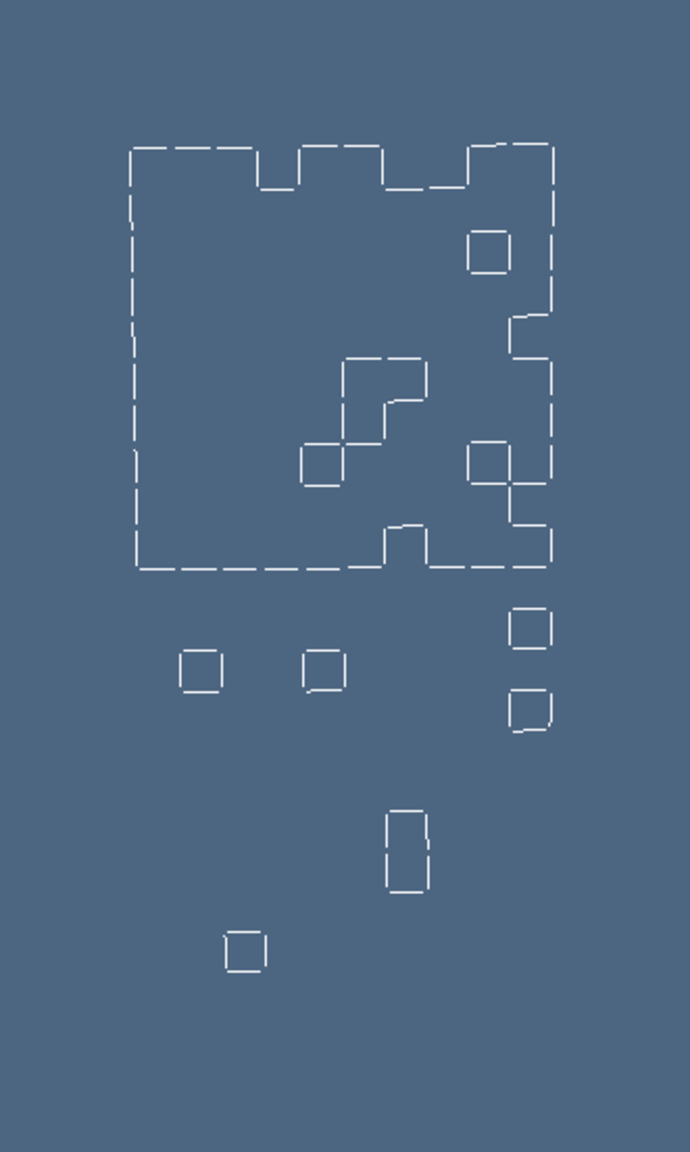
\includegraphics[height=0.3\linewidth,width=0.16\linewidth]{images/morph-chain1D1} 
   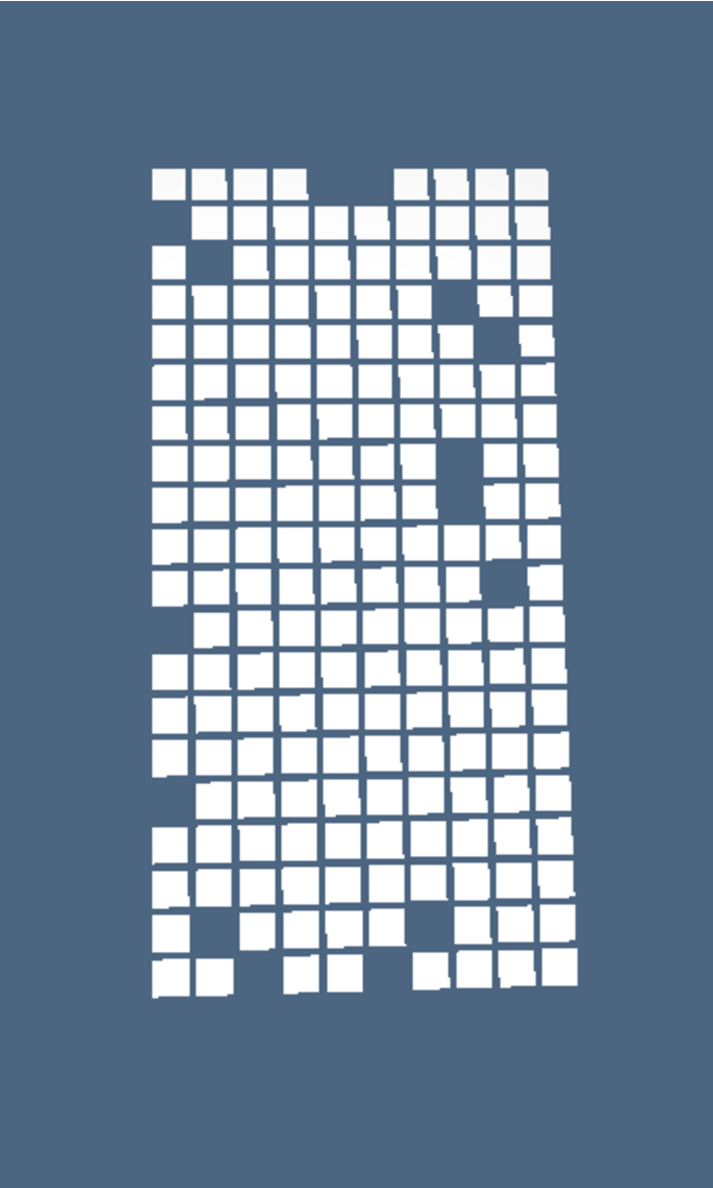
\includegraphics[height=0.3\linewidth,width=0.16\linewidth]{images/morph-chain2D2} 
   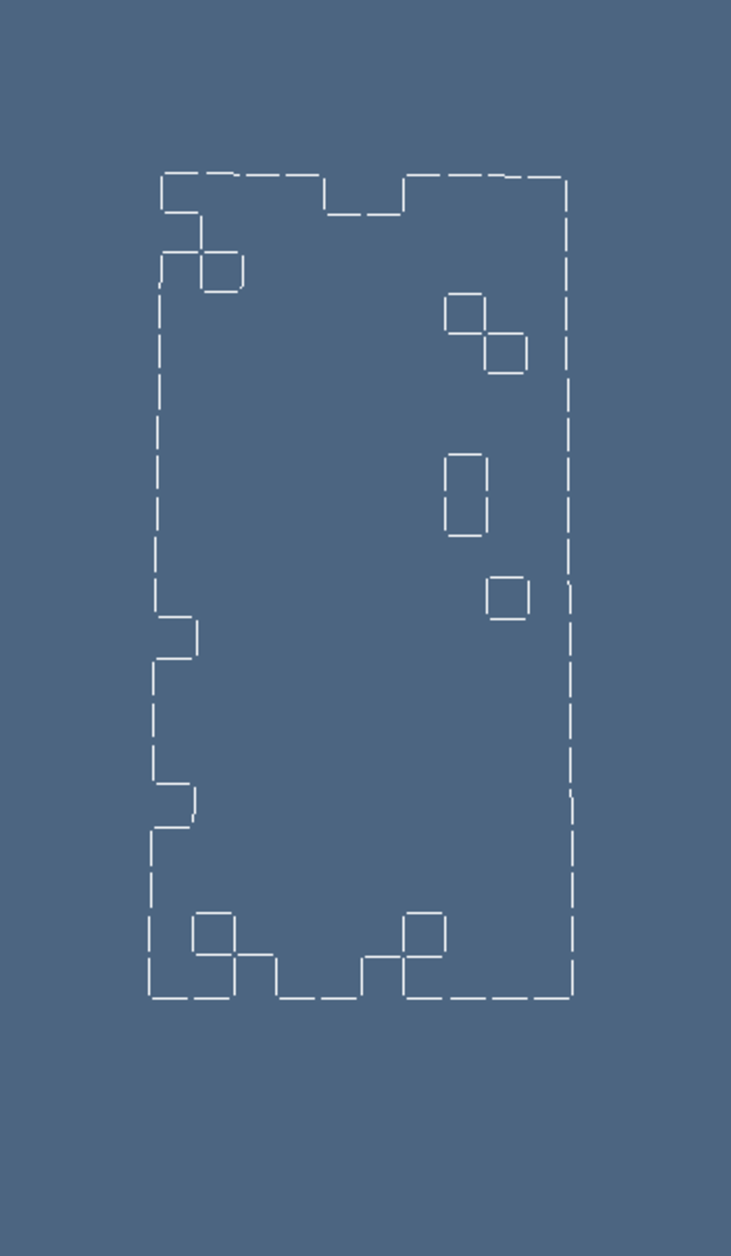
\includegraphics[height=0.3\linewidth,width=0.16\linewidth]{images/morph-chain1D2} 
   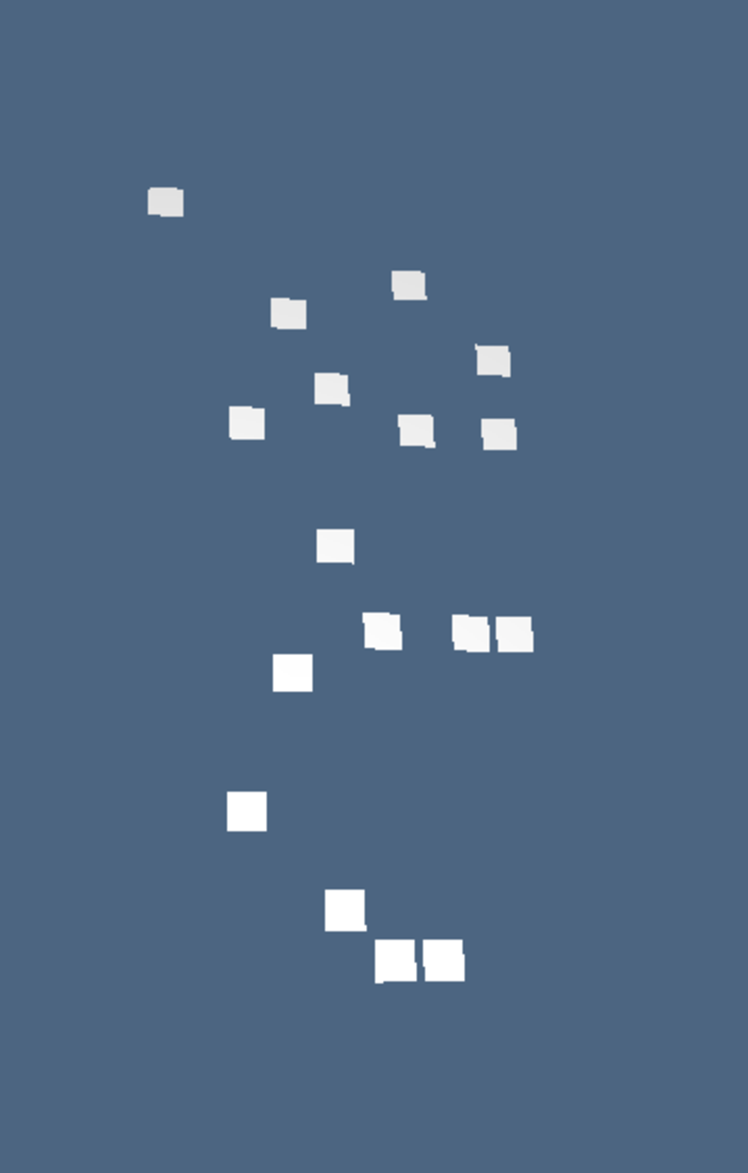
\includegraphics[height=0.3\linewidth,width=0.16\linewidth]{images/morph-chain2D3} 
   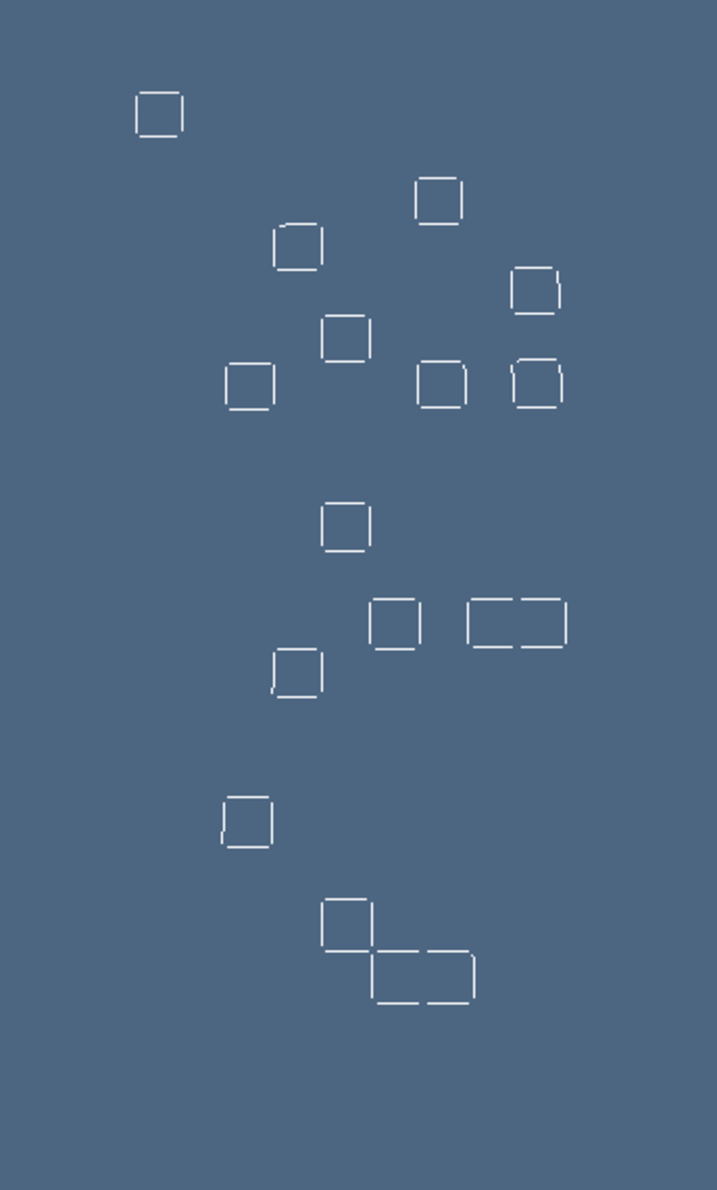
\includegraphics[height=0.3\linewidth,width=0.16\linewidth]{images/morph-chain1D3} 
   \caption{example caption}
   \label{fig:morph}
\end{figure}


\section{The bulk of morphological imaging}

The main part of the implementation of our algebraic construction of morphological operators on $d$-images is given in this section. First we introduce two generalized incidence operators, respectively named \emph{$\mathcal{U}_d$}, which stands for \emph{Upper}, and \emph{$\mathcal{L}_d$}, which stands for \emph{Lower}. Then we implement the standard morphological operators of Dilation (\emph{$\mathcal{D}_d$}), Erosion (\emph{$\mathcal{E}_d$}), Opening (\emph{$\mathcal{O}_d$}), and Closing (\emph{$\mathcal{C}_d$}).

\subsection{``Down'' and ``Up'' operators on Chains}

The Up and Down incidence operators are defined as mapping $d$-cells to $(d+1)$- and $(d+1)$-cells that, respectively, share vertices with them:
\[
\mathcal{U}_d : C_d \to C_{d+1}, \qquad \mathcal{D}_d : C_d \to C_{d-1}.
\]

Remembering that the characteristic matrix $M_d$ corresponds to the mapping from vertices to $d$-cells, we have
\[
[\mathcal{U}_d] = M_{d+1}\,M_d^t, \qquad [\mathcal{D}_d] = M_{d-1}\,M_d^t.
\]

\paragraph{Down and Up operators} Just consider that the characteristic matrices $M_{d-1},M_{d},M_{d+1}$,  stored in position $d-1$, $d$, and $d+1$ of the \texttt{skeletons} array, respectively provide the subsets of vertices of proper dimensions incising on each cell. They are used to compute the topological incidence operators, according to the paper~\cite{Dicarlo:2014:TNL:2543138.2543294}.

%-------------------------------------------------------------------------------
\begin{flushleft} \small
\begin{minipage}{\linewidth} \label{scrap17}
\protect\makebox[0ex][r]{\NWtarget{nuweb11}{\rule{0ex}{0ex}}\hspace{1em}}$\langle\,$Down and Up operators\nobreak\ {\footnotesize 11}$\,\rangle\equiv$
\vspace{-1ex}
\begin{list}{}{} \item
\mbox{}\verb@def larDown(skeletons,d):@\\
\mbox{}\verb@   """ Down operator, to multiply a d-chain and return the incident (d-1)-chain """@\\
\mbox{}\verb@   csrMd = csrCreate(skeletons[d])@\\
\mbox{}\verb@   csrMinus = csrCreate(skeletons[d-1])@\\
\mbox{}\verb@   csrDown = matrixProduct(csrMinus,csrTranspose(csrMd))@\\
\mbox{}\verb@   return csrDown@\\
\mbox{}\verb@   @\\
\mbox{}\verb@def larUp(skeletons,d):@\\
\mbox{}\verb@   """ Up operator, to multiply a d-chain and return the incident (d+1)-chain """@\\
\mbox{}\verb@   csrMd = csrCreate(skeletons[d])@\\
\mbox{}\verb@   csrPlus = csrCreate(skeletons[d+1])@\\
\mbox{}\verb@   csrUp = matrixProduct(csrPlus,csrTranspose(csrMd))@\\
\mbox{}\verb@   return csrUp   @\\
\mbox{}\verb@@{\NWsep}
\end{list}
\vspace{-1ex}
\footnotesize\addtolength{\baselineskip}{-1ex}
\begin{list}{}{\setlength{\itemsep}{-\parsep}\setlength{\itemindent}{-\leftmargin}}
\item \NWtxtMacroRefIn\ \NWlink{nuweb14e}{14e}.
\end{list}
\end{minipage}\\[4ex]
\end{flushleft}
%-------------------------------------------------------------------------------

\paragraph{The $\mathcal{UUD}$ operator}
A generic $\mathcal{UUD}: C_{d-1} \to C_{d}$ operator is given to be associated with the boundary $\partial_2$, in order to return the $\mathcal{ERO}\cup\mathcal{DIL}$ (TODO:correct) of a $d$-chain.

%-------------------------------------------------------------------------------
\begin{flushleft} \small
\begin{minipage}{\linewidth} \label{scrap18}
\protect\makebox[0ex][r]{\NWtarget{nuweb12a}{\rule{0ex}{0ex}}\hspace{1em}}$\langle\,$UUD operator: maps Down-UP-UP its input chains\nobreak\ {\footnotesize 12a}$\,\rangle\equiv$
\vspace{-1ex}
\begin{list}{}{} \item
\mbox{}\verb@def UUD(skeletons,d):@\\
\mbox{}\verb@   """ Compute the morphological operator UUP.@\\
\mbox{}\verb@      Return a CSR matrix to be applied to the coordinate representation of a chain@\\
\mbox{}\verb@   """ @\\
\mbox{}\verb@   D = larDown(skeletons,d)@\\
\mbox{}\verb@   U1 = larUp(skeletons,d-1)@\\
\mbox{}\verb@   U2 = larUp(skeletons,d)@\\
\mbox{}\verb@   UUDout = matrixProduct(U2,matrixProduct(U1,D))@\\
\mbox{}\verb@   return D,U1,U2,UUDout@\\
\mbox{}\verb@@{\NWsep}
\end{list}
\vspace{-1ex}
\footnotesize\addtolength{\baselineskip}{-1ex}
\begin{list}{}{\setlength{\itemsep}{-\parsep}\setlength{\itemindent}{-\leftmargin}}
\item \NWtxtMacroRefIn\ \NWlink{nuweb14e}{14e}.
\end{list}
\end{minipage}\\[4ex]
\end{flushleft}
%-------------------------------------------------------------------------------

A pair of similar function \texttt{testAlgebraicMorphology} and \texttt{testAlgebraicMorphologyStepByStep} are given here, both accepting the same (redundant) inputs, in order to test our algebraic approach to mathematical morphology. In particular: 

%\item
%\texttt{solid} is the LAR model (i.e.~the pair (\texttt{V},\texttt{CV})) of the original image;
%\item
%\texttt{b_rep} is the LAR model of its boundary (\texttt{V},\texttt{BV});
%\item
%\texttt{chain} is the $d$-chain of the image, given as the list of indices of $(d-1)$-cells within the boundary's $(d-1)$-chain;
%\item
%\texttt{imageVerts} 
%\item
%\texttt{skeletons} 

%-------------------------------------------------------------------------------
\begin{flushleft} \small
\begin{minipage}{\linewidth} \label{scrap19}
\protect\makebox[0ex][r]{\NWtarget{nuweb12b}{\rule{0ex}{0ex}}\hspace{1em}}$\langle\,$Testing the algebraic morphology\nobreak\ {\footnotesize 12b}$\,\rangle\equiv$
\vspace{-1ex}
\begin{list}{}{} \item
\mbox{}\verb@def testAlgebraicMorphology (solid, b_rep, chain, imageVerts, skeletons):@\\
\mbox{}\verb@   d = len(skeletons)-1@\\
\mbox{}\verb@   D,U1,U2,csrMorphOp = UUD(skeletons,d-1)@\\
\mbox{}\verb@   outputChain = chainTransform(skeletons,1,chain,csrMorphOp,d)@\\
\mbox{}\verb@   chainLAR = [cell for k,cell in enumerate(skeletons[d]) if k in outputChain]@\\
\mbox{}\verb@   model2 = (imageVerts,chainLAR)@\\
\mbox{}\verb@   return imageVerts,chainLAR@\\
\mbox{}\verb@@{\NWsep}
\end{list}
\vspace{-1ex}
\footnotesize\addtolength{\baselineskip}{-1ex}
\begin{list}{}{\setlength{\itemsep}{-\parsep}\setlength{\itemindent}{-\leftmargin}}
\item \NWtxtMacroRefIn\ \NWlink{nuweb14e}{14e}.
\end{list}
\end{minipage}\\[4ex]
\end{flushleft}
%-------------------------------------------------------------------------------

%-------------------------------------------------------------------------------
\begin{flushleft} \small
\begin{minipage}{\linewidth} \label{scrap20}
\protect\makebox[0ex][r]{\NWtarget{nuweb13a}{\rule{0ex}{0ex}}\hspace{1em}}$\langle\,$Testing the algebraic morphology method step-by-step\nobreak\ {\footnotesize 13a}$\,\rangle\equiv$
\vspace{-1ex}
\begin{list}{}{} \item
\mbox{}\verb@def testAlgebraicMorphologyStepByStep (solid, b_rep, chain, imageVerts, skeletons):@\\
\mbox{}\verb@   d = len(skeletons)-1@\\
\mbox{}\verb@   D,U1,U2,csrMorphOp = UUD(skeletons,d-1)@\\
\mbox{}\verb@   @\\
\mbox{}\verb@   VIEW(EXPLODE(1.5,1.5,1)(MKPOLS(solid)))@\\
\mbox{}\verb@   VIEW(COLOR(MAGENTA)(STRUCT(MKPOLS(b_rep))))@\\
\mbox{}\verb@   @\\
\mbox{}\verb@   outputChain = chainTransform(skeletons,d-1,chain,D,d-1)@\\
\mbox{}\verb@   chainLAR = [cell for k,cell in enumerate(skeletons[0]) if k in outputChain]@\\
\mbox{}\verb@   model0 = (imageVerts,chainLAR)@\\
\mbox{}\verb@   VIEW(COLOR(RED)(STRUCT(MKPOLS(model0))))@\\
\mbox{}\verb@   @\\
\mbox{}\verb@   M2 = csrCreate(skeletons[d])@\\
\mbox{}\verb@   @\\
\mbox{}\verb@   outputChain = chainTransform(skeletons,0,outputChain,M2,d)@\\
\mbox{}\verb@   chainLAR = [cell for k,cell in enumerate(skeletons[d]) if k in outputChain]@\\
\mbox{}\verb@   model2 = (imageVerts,chainLAR)@\\
\mbox{}\verb@   VIEW(COLOR(YELLOW)(STRUCT(MKPOLS(model2))))@\\
\mbox{}\verb@   @\\
\mbox{}\verb@   return imageVerts,chainLAR@\\
\mbox{}\verb@@{\NWsep}
\end{list}
\vspace{-1ex}
\footnotesize\addtolength{\baselineskip}{-1ex}
\begin{list}{}{\setlength{\itemsep}{-\parsep}\setlength{\itemindent}{-\leftmargin}}
\item \NWtxtMacroRefIn\ \NWlink{nuweb14e}{14e}.
\end{list}
\end{minipage}\\[4ex]
\end{flushleft}
%-------------------------------------------------------------------------------

\paragraph{Boundary chain mapping}
The function \texttt{chainTransform} takes as input a \texttt{chain} of dimension \texttt{d} (actually the boundary of a chain of dimension $d+1$), the \texttt{skeletons} array of \texttt{BRC} representations of matrices $M_k$ ($0\leq k\leq d+1$), and the number $n$ that $(d+1)$-cells resulting by multiplication with the operator's matrix \texttt{csrMatrix} must ahare with they incident $d$-cells in order to be included in the output of the considered algebraic morphology operator.

%-------------------------------------------------------------------------------
\begin{flushleft} \small
\begin{minipage}{\linewidth} \label{scrap21}
\protect\makebox[0ex][r]{\NWtarget{nuweb13b}{\rule{0ex}{0ex}}\hspace{1em}}$\langle\,$csrMatrix*chain product and interpretation\nobreak\ {\footnotesize 13b}$\,\rangle\equiv$
\vspace{-1ex}
\begin{list}{}{} \item
\mbox{}\verb@@\\
\mbox{}\verb@def chainTransform(skeletons,d,chain,csrMatrix,n):@\\
\mbox{}\verb@   # n: number of vertices shared in the incidence relation@\\
\mbox{}\verb@   cellNumber = len(skeletons[d])@\\
\mbox{}\verb@   csrChain = scipy.sparse.csr_matrix((cellNumber,1))@\\
\mbox{}\verb@   for h in chain: csrChain[h,0] = 1@\\
\mbox{}\verb@   cooOutChain = matrixProduct(csrMatrix, csrChain).tocoo()@\\
\mbox{}\verb@   outChain = [cooOutChain.row[h]@\\
\mbox{}\verb@      for h,val in enumerate(cooOutChain.data) if int(val) >= n]@\\
\mbox{}\verb@   return outChain @\\
\mbox{}\verb@@{\NWsep}
\end{list}
\vspace{-1ex}
\footnotesize\addtolength{\baselineskip}{-1ex}
\begin{list}{}{\setlength{\itemsep}{-\parsep}\setlength{\itemindent}{-\leftmargin}}
\item \NWtxtMacroRefIn\ \NWlink{nuweb14e}{14e}.
\end{list}
\end{minipage}\\[4ex]
\end{flushleft}
%-------------------------------------------------------------------------------


\paragraph{Example}

%-------------------------------------------------------------------------------
\begin{flushleft} \small
\begin{minipage}{\linewidth} \label{scrap22}
\protect\makebox[0ex][r]{\NWtarget{nuweb14a}{\rule{0ex}{0ex}}\hspace{1em}}$\langle\,$Algebraic dilation minus erosion\nobreak\ {\footnotesize 14a}$\,\rangle\equiv$
\vspace{-1ex}
\begin{list}{}{} \item
\mbox{}\verb@D1 = larDown(skeletons,1)@\\
\mbox{}\verb@U0 = larUp(skeletons,0)@\\
\mbox{}\verb@U1 = larUp(skeletons,1)@\\
\mbox{}\verb@UUD1 = UUD(skeletons,1)@\\
\mbox{}\verb@@{\NWsep}
\end{list}
\vspace{-1ex}
\footnotesize\addtolength{\baselineskip}{-1ex}
\begin{list}{}{\setlength{\itemsep}{-\parsep}\setlength{\itemindent}{-\leftmargin}}
\item {\NWtxtMacroNoRef}.
\end{list}
\end{minipage}\\[4ex]
\end{flushleft}
%-------------------------------------------------------------------------------



\subsection{Maximal ($d-2$)-chain extraction}


%-------------------------------------------------------------------------------
\begin{flushleft} \small
\begin{minipage}{\linewidth} \label{scrap23}
\protect\makebox[0ex][r]{\NWtarget{nuweb14b}{\rule{0ex}{0ex}}\hspace{1em}}$\langle\,$Extract the maximal ($d-2$)-chain from a ($d-1$)-chain\nobreak\ {\footnotesize 14b}$\,\rangle\equiv$
\vspace{-1ex}
\begin{list}{}{} \item
\mbox{}\verb@@\\
\mbox{}\verb@@\\
\mbox{}\verb@@{\NWsep}
\end{list}
\vspace{-1ex}
\footnotesize\addtolength{\baselineskip}{-1ex}
\begin{list}{}{\setlength{\itemsep}{-\parsep}\setlength{\itemindent}{-\leftmargin}}
\item {\NWtxtMacroNoRef}.
\end{list}
\end{minipage}\\[4ex]
\end{flushleft}
%-------------------------------------------------------------------------------

\subsection{($d-1$)-Star of a ($d-2$)-chain computation}

%-------------------------------------------------------------------------------
\begin{flushleft} \small
\begin{minipage}{\linewidth} \label{scrap24}
\protect\makebox[0ex][r]{\NWtarget{nuweb14c}{\rule{0ex}{0ex}}\hspace{1em}}$\langle\,$Compute the ($d-1$)-star of a ($d-2$)-chain\nobreak\ {\footnotesize 14c}$\,\rangle\equiv$
\vspace{-1ex}
\begin{list}{}{} \item
\mbox{}\verb@@\\
\mbox{}\verb@@\\
\mbox{}\verb@@{\NWsep}
\end{list}
\vspace{-1ex}
\footnotesize\addtolength{\baselineskip}{-1ex}
\begin{list}{}{\setlength{\itemsep}{-\parsep}\setlength{\itemindent}{-\leftmargin}}
\item {\NWtxtMacroNoRef}.
\end{list}
\end{minipage}\\[4ex]
\end{flushleft}
%-------------------------------------------------------------------------------


\subsection{$d$-Star of a $(d-1)$-chain computation}

%-------------------------------------------------------------------------------
\begin{flushleft} \small
\begin{minipage}{\linewidth} \label{scrap25}
\protect\makebox[0ex][r]{\NWtarget{nuweb14d}{\rule{0ex}{0ex}}\hspace{1em}}$\langle\,$Compute the d-star of a ($d-1$)-chain\nobreak\ {\footnotesize 14d}$\,\rangle\equiv$
\vspace{-1ex}
\begin{list}{}{} \item
\mbox{}\verb@@\\
\mbox{}\verb@@\\
\mbox{}\verb@@{\NWsep}
\end{list}
\vspace{-1ex}
\footnotesize\addtolength{\baselineskip}{-1ex}
\begin{list}{}{\setlength{\itemsep}{-\parsep}\setlength{\itemindent}{-\leftmargin}}
\item {\NWtxtMacroNoRef}.
\end{list}
\end{minipage}\\[4ex]
\end{flushleft}
%-------------------------------------------------------------------------------


\subsection{Dilation and erosion computation}



\subsection{Opening and closing computation}




\section{Exporting the \texttt{morph} module}

\paragraph{Exporting the morph module}
%-------------------------------------------------------------------------------
\begin{flushleft} \small \label{scrap26}
\protect\makebox[0ex][r]{\NWtarget{nuweb14e}{\rule{0ex}{0ex}}\hspace{1em}}\verb@"larlib/larlib/morph.py"@\nobreak\ {\footnotesize 14e }$\equiv$
\vspace{-1ex}
\begin{list}{}{} \item
\mbox{}\verb@""" LAR implementation of morphological operators on multidimensional images."""@\\
\mbox{}\verb@@\hbox{$\langle\,$Initial import of modules\nobreak\ {\footnotesize \NWlink{nuweb15}{15}}$\,\rangle$}\verb@@\\
\mbox{}\verb@@\hbox{$\langle\,$Generation of random image\nobreak\ {\footnotesize \NWlink{nuweb2a}{2a}}$\,\rangle$}\verb@@\\
\mbox{}\verb@@\hbox{$\langle\,$Save and restore data object from file\nobreak\ {\footnotesize \NWlink{nuweb6}{6}}$\,\rangle$}\verb@@\\
\mbox{}\verb@@\hbox{$\langle\,$Save or restore the chain complex of multidimensional image\nobreak\ {\footnotesize \NWlink{nuweb7a}{7a}}$\,\rangle$}\verb@@\\
\mbox{}\verb@@\hbox{$\langle\,$Tuples to integers mapping\nobreak\ {\footnotesize \NWlink{nuweb5a}{5a}}$\,\rangle$}\verb@@\\
\mbox{}\verb@@\hbox{$\langle\,$Generation of a masking window\nobreak\ {\footnotesize \NWlink{nuweb3b}{3b}}$\,\rangle$}\verb@@\\
\mbox{}\verb@@\hbox{$\langle\,$Characteristic matrices of multidimensional image\nobreak\ {\footnotesize \NWlink{nuweb7b}{7b}}$\,\rangle$}\verb@@\\
\mbox{}\verb@@\hbox{$\langle\,$CSR matrices of boundary operators\nobreak\ {\footnotesize \NWlink{nuweb9a}{9a}}$\,\rangle$}\verb@@\\
\mbox{}\verb@@\hbox{$\langle\,$csrMatrix*chain product and interpretation\nobreak\ {\footnotesize \NWlink{nuweb13b}{13b}}$\,\rangle$}\verb@@\\
\mbox{}\verb@@\hbox{$\langle\,$Pyplasm visualisation of an image chain\nobreak\ {\footnotesize \NWlink{nuweb10b}{10b}}$\,\rangle$}\verb@@\\
\mbox{}\verb@@\hbox{$\langle\,$Boundary of image chain computation\nobreak\ {\footnotesize \NWlink{nuweb9b}{9b}}$\,\rangle$}\verb@@\\
\mbox{}\verb@@\hbox{$\langle\,$Down and Up operators\nobreak\ {\footnotesize \NWlink{nuweb11}{11}}$\,\rangle$}\verb@@\\
\mbox{}\verb@@\hbox{$\langle\,$UUD operator: maps Down-UP-UP its input chains\nobreak\ {\footnotesize \NWlink{nuweb12a}{12a}}$\,\rangle$}\verb@@\\
\mbox{}\verb@@\hbox{$\langle\,$Testing the algebraic morphology method step-by-step\nobreak\ {\footnotesize \NWlink{nuweb13a}{13a}}$\,\rangle$}\verb@ @\\
\mbox{}\verb@@\hbox{$\langle\,$Testing the algebraic morphology\nobreak\ {\footnotesize \NWlink{nuweb12b}{12b}}$\,\rangle$}\verb@ @\\
\mbox{}\verb@@{\NWsep}
\end{list}
\vspace{-2ex}
\end{flushleft}
%-------------------------------------------------------------------------------

The set of importing commends needed by test files in this module is given in the macro below.

%-------------------------------------------------------------------------------
\begin{flushleft} \small
\begin{minipage}{\linewidth} \label{scrap27}
\protect\makebox[0ex][r]{\NWtarget{nuweb15}{\rule{0ex}{0ex}}\hspace{1em}}$\langle\,$Initial import of modules\nobreak\ {\footnotesize 15}$\,\rangle\equiv$
\vspace{-1ex}
\begin{list}{}{} \item
\mbox{}\verb@""" Initial import of modules """@\\
\mbox{}\verb@from larlib import *@\\
\mbox{}\verb@import scipy.misc, numpy, pickle@\\
\mbox{}\verb@from numpy.random import randint@\\
\mbox{}\verb@@{\NWsep}
\end{list}
\vspace{-1ex}
\footnotesize\addtolength{\baselineskip}{-1ex}
\begin{list}{}{\setlength{\itemsep}{-\parsep}\setlength{\itemindent}{-\leftmargin}}
\item \NWtxtMacroRefIn\ \NWlink{nuweb14e}{14e}\NWlink{nuweb16}{, 16}.
\end{list}
\end{minipage}\\[4ex]
\end{flushleft}
%-------------------------------------------------------------------------------


\section{Morphological operations examples}

\subsection{2D image masking and boundary computation}

\paragraph{Test example}

The \texttt{larcc.morph} API is used here to generate a random black and white image, with an \emph{image segment} selected and extracted by masking, then colored in middle grey, and exported to an image file.  
The \texttt{shape} and \texttt{structure} variables must contain two tuples, of equal \texttt{len}, of powers of 2, used toy define the size of random blocks in the generated image. The \texttt{window} variable is used to define the portion of the image where the \emph{segmentChain} of white pixels (or voxels, for 3-images) is computed.

%------------------------------------------------------------------
\begin{flushleft} \small
\begin{minipage}{\linewidth} \label{scrap28}
\protect\makebox[0ex][r]{\NWtarget{nuweb16}{\rule{0ex}{0ex}}\hspace{1em}}\verb@"test/py/morph/test01.py"@\nobreak\ {\footnotesize 16 }$\equiv$
\vspace{-1ex}
\begin{list}{}{} \item
\mbox{}\verb@@\\
\mbox{}\verb@@\hbox{$\langle\,$Initial import of modules\nobreak\ {\footnotesize \NWlink{nuweb15}{15}}$\,\rangle$}\verb@@\\
\mbox{}\verb@@\\
\mbox{}\verb@shape = 64,64@\\
\mbox{}\verb@structure = 8,8@\\
\mbox{}\verb@assert len(shape) == len(structure)@\\
\mbox{}\verb@imageVerts = larImageVerts(shape)@\\
\mbox{}\verb@_, skeletons, operators = imageChainComplex (shape)@\\
\mbox{}\verb@image_array = randomImage(shape, structure, 0.05)@\\
\mbox{}\verb@minPoint, maxPoint = (0,0), (64,64)@\\
\mbox{}\verb@window = minPoint, maxPoint@\\
\mbox{}\verb@segmentChain = setMaskWindow(window,image_array)@\\
\mbox{}\verb@   @\\
\mbox{}\verb@solid = visImageChain (shape,segmentChain, imageVerts, skeletons)@\\
\mbox{}\verb@b_rep,boundaryChain = imageChainBoundary(shape, operators)(2)(segmentChain)@\\
\mbox{}\verb@@\\
\mbox{}\verb@stepwiseTest = True@\\
\mbox{}\verb@if stepwiseTest:@\\
\mbox{}\verb@   model = testAlgebraicMorphologyStepByStep(solid, b_rep, @\\
\mbox{}\verb@            boundaryChain, imageVerts, skeletons)@\\
\mbox{}\verb@else:@\\
\mbox{}\verb@   model = testAlgebraicMorphology(solid, b_rep, @\\
\mbox{}\verb@            boundaryChain, imageVerts, skeletons)@\\
\mbox{}\verb@VIEW(STRUCT(MKPOLS(model)))@\\
\mbox{}\verb@@\\
\mbox{}\verb@V = model[0]@\\
\mbox{}\verb@M = AA(tuple)(model[1])@\\
\mbox{}\verb@S = AA(tuple)(solid[1])@\\
\mbox{}\verb@B = AA(tuple)(b_rep[1])@\\
\mbox{}\verb@D = list(set(S).union(M))@\\
\mbox{}\verb@E = list(set(S).difference(M))@\\
\mbox{}\verb@M,S,B,D,E = (AA(AA(list)))([M,S,B,D,E])@\\
\mbox{}\verb@M2 = STRUCT(MKPOLS((V,M)))@\\
\mbox{}\verb@S2 = STRUCT(MKPOLS((V,S)))@\\
\mbox{}\verb@@\\
\mbox{}\verb@S2 = COLOR(CYAN)(STRUCT(MKPOLS((V,S))))@\\
\mbox{}\verb@B1 = COLOR(MAGENTA)(STRUCT(MKPOLS((V,B))))@\\
\mbox{}\verb@D2 = COLOR(YELLOW)(STRUCT(MKPOLS((V,D))))@\\
\mbox{}\verb@E2 = COLOR(WHITE)(STRUCT(MKPOLS((V,E))))@\\
\mbox{}\verb@VIEW(STRUCT([D2,S2,E2,B1]))@\\
\mbox{}\verb@@\\
\mbox{}\verb@VIEW(STRUCT([D2,S2,B1]))@\\
\mbox{}\verb@VIEW(STRUCT([S2,E2,B1]))@\\
\mbox{}\verb@@\\
\mbox{}\verb@@{\NWsep}
\end{list}
\vspace{-2ex}
\end{minipage}\\[4ex]
\end{flushleft}
%------------------------------------------------------------------

%A0 = matrix([
%[0,2,0],
%[4,0,0],
%[0,0,2],
%])
%B0 = matrix([
%[0,1,0],
%[1,0,0],
%[0,0,1],
%])
%A1 = matrix([
%[0,10,0],
%[0,11,0],
%[5,0,12],
%])
%B1 = matrix([
%[0,1,0],
%[0,1,0],
%[1,0,1],
%])


%===============================================================================
\appendix
\section{Utilities}

\subsection{Importing a generic module}
First we define a parametric macro to allow the importing of \texttt{larcc} modules from the project repository \texttt{lib/py/}. When the user needs to import some project's module, she may call this macro as done in Section~\ref{sec:lar2psm}.
%------------------------------------------------------------------
\begin{flushleft} \small
\begin{minipage}{\linewidth} \label{scrap29}
\protect\makebox[0ex][r]{\NWtarget{nuweb17a}{\rule{0ex}{0ex}}\hspace{1em}}$\langle\,$Import the module\nobreak\ {\footnotesize 17a}$\,\rangle\equiv$
\vspace{-1ex}
\begin{list}{}{} \item
\mbox{}\verb@import @@1\verb@@\\
\mbox{}\verb@from @@1\verb@ import *@\\
\mbox{}\verb@@{\NWsep}
\end{list}
\vspace{-1ex}
\footnotesize\addtolength{\baselineskip}{-1ex}
\begin{list}{}{\setlength{\itemsep}{-\parsep}\setlength{\itemindent}{-\leftmargin}}
\item \NWtxtMacroRefIn\ \NWlink{nuweb17b}{17b}.
\end{list}
\end{minipage}\\[4ex]
\end{flushleft}
%------------------------------------------------------------------

\paragraph{Importing a module} A function used to import a generic \texttt{lacccc} module within the current environment is also useful.
%------------------------------------------------------------------
\begin{flushleft} \small
\begin{minipage}{\linewidth} \label{scrap30}
\protect\makebox[0ex][r]{\NWtarget{nuweb17b}{\rule{0ex}{0ex}}\hspace{1em}}$\langle\,$Function to import a generic module\nobreak\ {\footnotesize 17b}$\,\rangle\equiv$
\vspace{-1ex}
\begin{list}{}{} \item
\mbox{}\verb@def importModule(moduleName):@\\
\mbox{}\verb@   @\hbox{$\langle\,$Import the module\nobreak\ ({\footnotesize \NWtarget{nuweb17c}{17c}\label{scrap31}
 }\mbox{}\verb@moduleName@ ) {\footnotesize \NWlink{nuweb17a}{17a}}$\,\rangle$}\verb@@\\
\mbox{}\verb@@{\NWsep}
\end{list}
\vspace{-1ex}
\footnotesize\addtolength{\baselineskip}{-1ex}
\begin{list}{}{\setlength{\itemsep}{-\parsep}\setlength{\itemindent}{-\leftmargin}}
\item {\NWtxtMacroNoRef}.
\end{list}
\end{minipage}\\[4ex]
\end{flushleft}
%------------------------------------------------------------------


\bibliographystyle{amsalpha}
\bibliography{morph}

\end{document}
